%%%%%%%%%%%%%%%%%%%%%%%%%%%%%%%%%
%Preamble
%%%%%%%%%%%%%%%%%%%%%%%%%%%%%%%%%

\PassOptionsToPackage{usenames, dvipsnames}{xcolor}

\documentclass[11pt, a4paper, table]{article}
\usepackage[english]{babel}
\usepackage[margin=1in]{geometry}
\usepackage[ruled, vlined]{algorithm2e}

\usepackage{amsfonts}
\usepackage{setspace,graphicx,epstopdf,amsmath}
\usepackage{marginnote, datetime, url, enumitem, subfigure}
\usepackage[capposition=top]{floatrow}
\usepackage{placeins}

%Journal Style
%JFE looks nice, JF looks awful
	\usepackage{amsthm}
	\usepackage{jfe}

%Bibliography Stuff
	%Use natbib even though it's old because it's compliant with journal styles
	%Actual bibliography style etc are specified where you actually want it
	\usepackage{natbib}

%Fluff
	\linespread{1.3}

%Neural Network Packages
	\usepackage{neuralnetwork}
	\usepackage{xpatch}
	\makeatletter
	% \linklayers have \nn@lastnode instead of \lastnode,
	% patch it to replace the former with the latter, and similar for thisnode
	\xpatchcmd{\linklayers}{\nn@lastnode}{\lastnode}{}{}
	\xpatchcmd{\linklayers}{\nn@thisnode}{\thisnode}{}{}
	\makeatother
	
%Regression Tree
	\usepackage{tikz,forest}
	\usetikzlibrary{arrows.meta}
	
	\forestset{
		.style={
			for tree={
				base=bottom,
				child anchor=north,
				align=center,
				s sep+=1cm,
				straight edge/.style={
					edge path={\noexpand\path[\forestoption{edge},thick,-{Latex}] 
						(!u.parent anchor) -- (.child anchor);}
				},
				if n children={0}
				{tier=word, draw, thick, rectangle}
				{draw, diamond, thick, aspect=2},
				if n=1{%
					edge path={\noexpand\path[\forestoption{edge},thick,-{Latex}] 
						(!u.parent anchor) -| (.child anchor) node[pos=.2, above] {Y};}
				}{
					edge path={\noexpand\path[\forestoption{edge},thick,-{Latex}] 
						(!u.parent anchor) -| (.child anchor) node[pos=.2, above] {N};}
				}
			}
		}
	}

\usepackage{lscape}
\usepackage{longtable}

%%TODONOTE commands
\usepackage[colorinlistoftodos]{todonotes}
\newcommand{\smalltodo}[2][] {\todo[caption={#2}, size=\scriptsize,%
	fancyline,#1]{\begin{spacing}{.5}#2\end{spacing}}}
\newcommand{\rhs}[2][]{\smalltodo[color=green!30,#1]{{\bf RS:} #2}}
%%

%Graphs
\usepackage{tikz}
\usepackage{pgfplots}
\usepackage[export]{adjustbox}

\graphicspath{{../Results/}}

\usepackage{multirow}
\usepackage{array}
\usepackage{multirow}
\usepackage{wrapfig}
\usepackage{float}
\usepackage{colortbl}
\usepackage{pdflscape}
\usepackage{tabu}
\usepackage{booktabs}
\usepackage{threeparttable}
\usepackage{threeparttablex}
\usepackage[normalem]{ulem}
\usepackage{makecell}
\usepackage{xcolor}

%Coloured Tables

%%%%%%%%%%%%%%%%%%%%%%%%%%%%%%
%%Title and other fluff, just before document start
%%%%%%%%%%%%%%%%%%%%%%%%%%%%%%

%Hyperref apparently is a big package and causes a lot of issues, so it's recommended to load this last

\usepackage{hyperref}

%Gets rid of the neon green boxes around boxes

\usepackage[]{xcolor}

\hypersetup{
	colorlinks,
	linkcolor = {red!50!black},
	citecolor = {blue!50!black},
	urlcolor = {blue!80!black}
}

\title{Evaluation of Machine Learning in Empirical Asset Pricing
\thanks{I acknowledge and thank David Frazier, my supervisor, Xueyan Zhao and Jun Sung Kim, my honours degree coordinators, as well as my fellow honours cohort for their support throughout the writing of this thesis. I would also like to acknowledge the work of \cite{gu_empirical_2018}, and in particular for their provision of the dataset which they constructed.}
}
\author{Ze Yu Zhong \\
Supervisor: David Frazier \\ 
Thesis submitted for the completion of the \\
Bachelor of Commerce (Honours) in Econometrics at \\
Monash University}

%%%%%%%%%%%%%%%%%%%%%%%%%%%%%%%
%%BEGIN DOCUMENT
%%%%%%%%%%%%%%%%%%%%%%%%%%%%%%%

\begin{document}

\section{Appendix}

\subsection{Data}

\subsection{Additional Results}

\subsubsection{Simulation Study}

%% Small Results
\begin{table}

\caption{\label{tab:}Top Models by MAE in Simulation Study}
\centering
\fontsize{8}{10}\selectfont
\begin{tabular}[t]{ccccc}
\toprule
\multicolumn{1}{c}{ } & \multicolumn{1}{c}{ } & \multicolumn{3}{c}{Test MAE} \\
\cmidrule(l{3pt}r{3pt}){3-5}
Corr & model & g1 & g2 & g3\\
\midrule
 & ELN.MAE & \textbf{0.034579} & 0.036195 & \textbf{0.035334}\\

 & RF.MAE & 0.035459 & \textbf{0.03542} & 0.03554\\

 & NN2.MAE & 0.03596 & 0.036921 & 0.036305\\

 & NN1.MAE & 0.035894 & 0.036834 & 0.036335\\

\multirow{-5}{*}{\centering\arraybackslash \rotatebox{90}{0.01}} & NN3.MAE & 0.035816 & 0.036934 & 0.036471\\
\cmidrule{1-5}
 & ELN.MSE & \textbf{0.034614} & 0.036276 & \textbf{0.035444}\\

 & RF.MAE & 0.035916 & \textbf{0.035643} & 0.036053\\

 & NN5.MAE & 0.037009 & 0.03727 & 0.037413\\

 & NN4.MSE & 0.037382 & 0.036897 & 0.037354\\

\multirow{-5}{*}{\centering\arraybackslash \rotatebox{90}{1}} & NN3.MAE & 0.037285 & 0.037038 & 0.037193\\
\bottomrule
\end{tabular}
\end{table}

\begin{table}

\caption{\label{tab:}Top Models by MSE in Simulation Study}
\centering
\fontsize{6}{8}\selectfont
\begin{tabular}[t]{ccccc}
\toprule
\multicolumn{1}{c}{ } & \multicolumn{1}{c}{ } & \multicolumn{3}{c}{Test MSE} \\
\cmidrule(l{3pt}r{3pt}){3-5}
Corr & model & g1 & g2 & g3\\
\midrule
 & ELN.MAE & \textbf{0.0026} & 0.0027 & \textbf{0.0026}\\

 & RF.MAE & 0.0026 & \textbf{0.0026} & 0.0026\\

 & NN2.MAE & 0.0027 & 0.0027 & 0.0027\\

 & NN1.MAE & 0.0027 & 0.0027 & 0.0027\\

\multirow{-5}{*}{\centering\arraybackslash \rotatebox{90}{0.01}} & NN3.MAE & 0.0027 & 0.0027 & 0.0027\\
\cmidrule{1-5}
 & ELN.MSE & \textbf{0.0026} & 0.0027 & \textbf{0.0026}\\

 & RF.MAE & 0.0027 & \textbf{0.0026} & 0.0027\\

 & NN5.MAE & 0.0028 & 0.0028 & 0.0028\\

 & NN3.MAE & 0.0028 & 0.0028 & 0.0028\\

\multirow{-5}{*}{\centering\arraybackslash \rotatebox{90}{1}} & NN4.MSE & 0.0028 & 0.0028 & 0.0028\\
\bottomrule
\end{tabular}
\end{table}

\newpage

%% Comprehensive Results
\begingroup\fontsize{6}{8}\selectfont

\begin{longtable}{ccccccccccc}
\toprule
\multicolumn{1}{c}{ } & \multicolumn{1}{c}{ } & \multicolumn{3}{c}{g1} & \multicolumn{3}{c}{g2} & \multicolumn{3}{c}{g3} \\
\cmidrule(l{3pt}r{3pt}){3-5} \cmidrule(l{3pt}r{3pt}){6-8} \cmidrule(l{3pt}r{3pt}){9-11}
model & Corr & Test MAE & Test MSE & Test $R^2$ & Test MAE & Test MSE & Test $R^2$ & Test MAE & Test MSE & Test $R^2$\\
\midrule
\endfirsthead
\multicolumn{11}{@{}l}{}\\
\toprule
\multicolumn{1}{c}{ } & \multicolumn{1}{c}{ } & \multicolumn{3}{c}{g1} & \multicolumn{3}{c}{g2} & \multicolumn{3}{c}{g3} \\
\cmidrule(l{3pt}r{3pt}){3-5} \cmidrule(l{3pt}r{3pt}){6-8} \cmidrule(l{3pt}r{3pt}){9-11}
model & Corr & Test MAE & Test MSE & Test $R^2$ & Test MAE & Test MSE & Test $R^2$ & Test MAE & Test MSE & Test $R^2$\\
\midrule
\endhead
\
\endfoot
\bottomrule
\endlastfoot
 & 0.01 & 0.036678 & 0.002740 & 0.008273 & 0.038255 & 0.002880 & -0.111788 & 0.037310 & 0.002795 & -0.032068\\
\cmidrule{2-11}
 & 0.10 & 0.036965 & 0.002765 & -0.011020 & 0.038580 & 0.002914 & -0.142944 & 0.037569 & 0.002817 & -0.054940\\
\cmidrule{2-11}
\multirow{-3}{*}{\centering\arraybackslash LM.MSE} & 1.00 & 0.042949 & 0.003414 & -0.438797 & 0.045376 & 0.003717 & -0.780953 & 0.043434 & 0.003469 & -0.488779\\
\cmidrule{1-11}
 & 0.01 & 0.036642 & 0.002737 & 0.009050 & 0.038348 & 0.002886 & -0.116369 & 0.037324 & 0.002797 & -0.035162\\
\cmidrule{2-11}
 & 0.10 & 0.036811 & 0.002755 & 0.002919 & 0.038745 & 0.002927 & -0.152580 & 0.037489 & 0.002810 & -0.047675\\
\cmidrule{2-11}
\multirow{-3}{*}{\centering\arraybackslash LM.MAE} & 1.00 & 0.042340 & 0.003344 & -0.393044 & 0.045342 & 0.003685 & -0.769955 & 0.043535 & 0.003468 & -0.544524\\
\cmidrule{1-11}
 & 0.01 & 0.034588 & 0.002566 & 0.140335 & 0.036223 & 0.002690 & 0.036877 & 0.035353 & 0.002623 & 0.099142\\
\cmidrule{2-11}
 & 0.10 & 0.034563 & 0.002564 & 0.144238 & 0.036183 & 0.002686 & 0.037258 & 0.035292 & 0.002617 & 0.100241\\
\cmidrule{2-11}
\multirow{-3}{*}{\centering\arraybackslash ELN.MSE} & 1.00 & 0.034614 & 0.002568 & 0.167184 & 0.036276 & 0.002698 & 0.037839 & 0.035444 & 0.002630 & 0.119875\\
\cmidrule{1-11}
 & 0.01 & 0.034579 & 0.002565 & 0.140982 & 0.036195 & 0.002688 & 0.039169 & 0.035334 & 0.002621 & 0.100442\\
\cmidrule{2-11}
 & 0.10 & 0.034558 & 0.002564 & 0.144627 & 0.036173 & 0.002688 & 0.038875 & 0.035285 & 0.002617 & 0.100919\\
\cmidrule{2-11}
\multirow{-3}{*}{\centering\arraybackslash ELN.MAE} & 1.00 & 0.034599 & 0.002567 & 0.167771 & 0.036305 & 0.002703 & 0.036583 & 0.035465 & 0.002631 & 0.118022\\
\cmidrule{1-11}
 & 0.01 & 0.035775 & 0.002671 & 0.063426 & 0.035718 & 0.002657 & 0.067615 & 0.035803 & 0.002661 & 0.070298\\
\cmidrule{2-11}
 & 0.10 & 0.035769 & 0.002665 & 0.066738 & 0.035684 & 0.002652 & 0.069139 & 0.035867 & 0.002670 & 0.062839\\
\cmidrule{2-11}
\multirow{-3}{*}{\centering\arraybackslash RF.MSE} & 1.00 & 0.036233 & 0.002698 & 0.068774 & 0.035989 & 0.002683 & 0.057103 & 0.036213 & 0.002695 & 0.069887\\
\cmidrule{1-11}
 & 0.01 & 0.035459 & 0.002643 & 0.083338 & 0.035420 & 0.002630 & 0.087653 & 0.035540 & 0.002645 & 0.086529\\
\cmidrule{2-11}
 & 0.10 & 0.035515 & 0.002649 & 0.081425 & 0.035489 & 0.002634 & 0.083405 & 0.035569 & 0.002644 & 0.081643\\
\cmidrule{2-11}
\multirow{-3}{*}{\centering\arraybackslash RF.MAE} & 1.00 & 0.035916 & 0.002675 & 0.087081 & 0.035643 & 0.002644 & 0.080965 & 0.036053 & 0.002679 & 0.075357\\
\cmidrule{1-11}
 & 0.01 & 0.036452 & 0.002722 & 0.016344 & 0.036768 & 0.002732 & -0.003917 & 0.036687 & 0.002738 & 0.009335\\
\cmidrule{2-11}
 & 0.10 & 0.036462 & 0.002719 & 0.020422 & 0.036776 & 0.002734 & -0.007259 & 0.036733 & 0.002737 & 0.002955\\
\cmidrule{2-11}
\multirow{-3}{*}{\centering\arraybackslash NN1.MSE} & 1.00 & 0.037545 & 0.002821 & -0.014452 & 0.037049 & 0.002764 & -0.014697 & 0.037459 & 0.002798 & -0.012469\\
\cmidrule{1-11}
 & 0.01 & 0.035960 & 0.002679 & 0.055814 & 0.036921 & 0.002747 & -0.015105 & 0.036305 & 0.002700 & 0.039371\\
\cmidrule{2-11}
 & 0.10 & 0.036082 & 0.002687 & 0.050698 & 0.037010 & 0.002750 & -0.020562 & 0.036322 & 0.002702 & 0.032303\\
\cmidrule{2-11}
\multirow{-3}{*}{\centering\arraybackslash NN1.MAE} & 1.00 & 0.037889 & 0.002834 & -0.043182 & 0.037979 & 0.002845 & -0.084075 & 0.037306 & 0.002793 & 0.002178\\
\cmidrule{1-11}
 & 0.01 & 0.037019 & 0.002785 & -0.021787 & 0.037320 & 0.002775 & -0.043354 & 0.037089 & 0.002774 & -0.017304\\
\cmidrule{2-11}
 & 0.10 & 0.036977 & 0.002765 & -0.021276 & 0.037009 & 0.002748 & -0.027538 & 0.036990 & 0.002758 & -0.020645\\
\cmidrule{2-11}
\multirow{-3}{*}{\centering\arraybackslash NN2.MSE} & 1.00 & 0.037536 & 0.002814 & -0.013978 & 0.036903 & 0.002752 & -0.005866 & 0.037516 & 0.002809 & -0.016934\\
\cmidrule{1-11}
 & 0.01 & 0.035894 & 0.002672 & 0.057743 & 0.036834 & 0.002740 & -0.007158 & 0.036335 & 0.002703 & 0.036305\\
\cmidrule{2-11}
 & 0.10 & 0.035890 & 0.002668 & 0.060310 & 0.036937 & 0.002750 & -0.017077 & 0.036270 & 0.002696 & 0.037157\\
\cmidrule{2-11}
\multirow{-3}{*}{\centering\arraybackslash NN2.MAE} & 1.00 & 0.037480 & 0.002814 & -0.009529 & 0.037715 & 0.002823 & -0.065390 & 0.037471 & 0.002804 & -0.010118\\
\cmidrule{1-11}
 & 0.01 & 0.036783 & 0.002757 & -0.006762 & 0.036840 & 0.002738 & -0.007525 & 0.037036 & 0.002764 & -0.020078\\
\cmidrule{2-11}
 & 0.10 & 0.036938 & 0.002761 & -0.015399 & 0.036852 & 0.002738 & -0.015106 & 0.036874 & 0.002757 & -0.004406\\
\cmidrule{2-11}
\multirow{-3}{*}{\centering\arraybackslash NN3.MSE} & 1.00 & 0.037424 & 0.002808 & -0.012964 & 0.036938 & 0.002754 & -0.006353 & 0.037420 & 0.002799 & -0.010348\\
\cmidrule{1-11}
 & 0.01 & 0.035816 & 0.002670 & 0.065432 & 0.036934 & 0.002749 & -0.016398 & 0.036471 & 0.002718 & 0.029948\\
\cmidrule{2-11}
 & 0.10 & 0.035893 & 0.002677 & 0.062002 & 0.036859 & 0.002741 & -0.011850 & 0.036200 & 0.002693 & 0.040611\\
\cmidrule{2-11}
\multirow{-3}{*}{\centering\arraybackslash NN3.MAE} & 1.00 & 0.037009 & 0.002774 & 0.021329 & 0.037270 & 0.002783 & -0.029644 & 0.037413 & 0.002792 & -0.008307\\
\cmidrule{1-11}
 & 0.01 & 0.036881 & 0.002759 & -0.020620 & 0.036856 & 0.002742 & -0.007715 & 0.037126 & 0.002775 & -0.026563\\
\cmidrule{2-11}
 & 0.10 & 0.036877 & 0.002761 & -0.014579 & 0.037221 & 0.002762 & -0.048711 & 0.036872 & 0.002748 & -0.008894\\
\cmidrule{2-11}
\multirow{-3}{*}{\centering\arraybackslash NN4.MSE} & 1.00 & 0.037382 & 0.002805 & -0.006481 & 0.036897 & 0.002751 & -0.005369 & 0.037354 & 0.002797 & -0.007739\\
\cmidrule{1-11}
 & 0.01 & 0.035935 & 0.002678 & 0.057720 & 0.036897 & 0.002749 & -0.010917 & 0.036708 & 0.002738 & 0.007046\\
\cmidrule{2-11}
 & 0.10 & 0.035828 & 0.002665 & 0.065041 & 0.036933 & 0.002749 & -0.019112 & 0.036273 & 0.002695 & 0.037704\\
\cmidrule{2-11}
\multirow{-3}{*}{\centering\arraybackslash NN4.MAE} & 1.00 & 0.037095 & 0.002779 & 0.019866 & 0.037323 & 0.002795 & -0.029377 & 0.037301 & 0.002787 & -0.001888\\
\cmidrule{1-11}
 & 0.01 & 0.037231 & 0.002785 & -0.049970 & 0.036931 & 0.002747 & -0.017002 & 0.037114 & 0.002772 & -0.021895\\
\cmidrule{2-11}
 & 0.10 & 0.037026 & 0.002767 & -0.032190 & 0.037176 & 0.002762 & -0.039436 & 0.036909 & 0.002757 & -0.011352\\
\cmidrule{2-11}
\multirow{-3}{*}{\centering\arraybackslash NN5.MSE} & 1.00 & 0.037364 & 0.002795 & -0.010495 & 0.036928 & 0.002755 & -0.005376 & 0.037475 & 0.002807 & -0.014974\\
\cmidrule{1-11}
 & 0.01 & 0.035888 & 0.002669 & 0.058579 & 0.036835 & 0.002738 & -0.008646 & 0.036685 & 0.002737 & 0.004643\\
\cmidrule{2-11}
 & 0.10 & 0.036038 & 0.002680 & 0.050976 & 0.036745 & 0.002727 & -0.004935 & 0.036484 & 0.002710 & 0.018192\\
\cmidrule{2-11}
\multirow{-3}{*}{\centering\arraybackslash NN5.MAE} & 1.00 & 0.037285 & 0.002794 & 0.002541 & 0.037038 & 0.002765 & -0.012729 & 0.037193 & 0.002775 & 0.002572\\
\cmidrule{1-11}
 & 0.01 & 0.037296 & 0.002798 & -0.043289 & 0.037227 & 0.002776 & -0.044764 & 0.037591 & 0.002818 & -0.062516\\
\cmidrule{2-11}
 & 0.10 & 0.037237 & 0.002795 & -0.031955 & 0.037134 & 0.002767 & -0.038255 & 0.037198 & 0.002785 & -0.030394\\
\cmidrule{2-11}
\multirow{-3}{*}{\centering\arraybackslash LSTM.MSE} & 1.00 & 0.038128 & 0.002851 & -0.082027 & 0.037382 & 0.002792 & -0.044243 & 0.037780 & 0.002830 & -0.044330\\
\cmidrule{1-11}
 & 0.01 & 0.037431 & 0.002805 & -0.056406 & 0.037337 & 0.002780 & -0.051854 & 0.037627 & 0.002817 & -0.067433\\
\cmidrule{2-11}
 & 0.10 & 0.037446 & 0.002804 & -0.062952 & 0.037118 & 0.002768 & -0.032544 & 0.037241 & 0.002793 & -0.033320\\
\cmidrule{2-11}
\multirow{-3}{*}{\centering\arraybackslash LSTM.MAE} & 1.00 & 0.038027 & 0.002846 & -0.061483 & 0.037415 & 0.002790 & -0.045506 & 0.037743 & 0.002825 & -0.045884\\
\cmidrule{1-11}
 & 0.01 & 0.038277 & 0.002882 & -0.132672 & 0.038460 & 0.002889 & -0.147390 & 0.042466 & 0.003311 & -0.486145\\
\cmidrule{2-11}
 & 0.10 & 0.038358 & 0.002895 & -0.140765 & 0.038479 & 0.002891 & -0.160062 & 0.042323 & 0.003291 & -0.473991\\
\cmidrule{2-11}
\multirow{-3}{*}{\centering\arraybackslash FFORMA.MSE} & 1.00 & 0.038875 & 0.002965 & -0.131239 & 0.038808 & 0.002933 & -0.165990 & 0.043013 & 0.003371 & -0.470954\\
\cmidrule{1-11}
 & 0.01 & 0.038755 & 0.002939 & -0.179748 & 0.038747 & 0.002918 & -0.174094 & 0.042989 & 0.003365 & -0.527909\\
\cmidrule{2-11}
 & 0.10 & 0.038936 & 0.002951 & -0.192793 & 0.038796 & 0.002946 & -0.175994 & 0.043097 & 0.003406 & -0.586375\\
\cmidrule{2-11}
\multirow{-3}{*}{\centering\arraybackslash FFORMA.MAE} & 1.00 & 0.039247 & 0.002972 & -0.163656 & 0.039387 & 0.002996 & -0.211619 & 0.043709 & 0.003448 & -0.526081\\
\cmidrule{1-11}
 & 0.01 & 0.038299 & 0.002900 & -0.128930 & 0.038489 & 0.002912 & -0.132518 & 0.039390 & 0.003016 & -0.204980\\
\cmidrule{2-11}
 & 0.10 & 0.038832 & 0.002935 & -0.181663 & 0.038435 & 0.002905 & -0.131874 & 0.039177 & 0.002993 & -0.190558\\
\cmidrule{2-11}
\multirow{-3}{*}{\centering\arraybackslash DeepAR} & 1.00 & 0.040535 & 0.003159 & -0.239142 & 0.038787 & 0.002952 & -0.144029 & 0.039692 & 0.003042 & -0.182365\\*
\end{longtable}
\endgroup{}

\FloatBarrier

%% Factor Analysis

\begin{figure}
	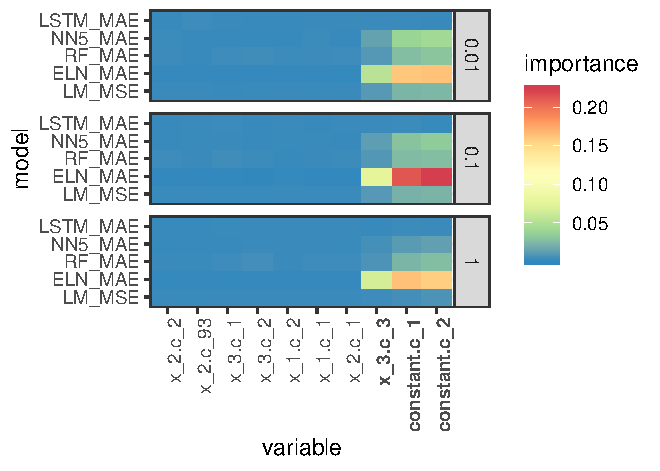
\includegraphics[]{../Results/simulation/graphics/simulation_g1_vi.pdf}
\end{figure}

\begin{figure}
	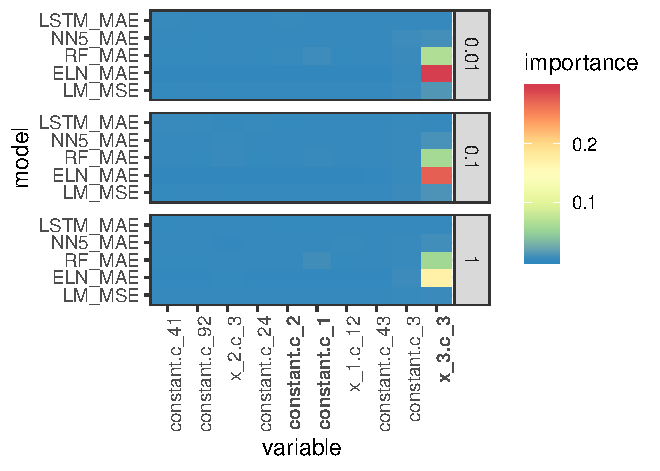
\includegraphics[]{../Results/simulation/graphics/simulation_g2_vi.pdf}
\end{figure}

\begin{figure}
	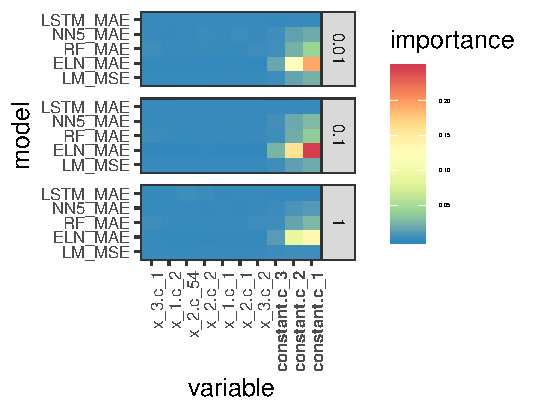
\includegraphics[]{../Results/simulation/graphics/simulation_g3_vi.pdf}
\end{figure}

%%%%%%%%%%%%%%%%%%%%
%% Random Forest Vimps
%% BC

\begin{figure}
	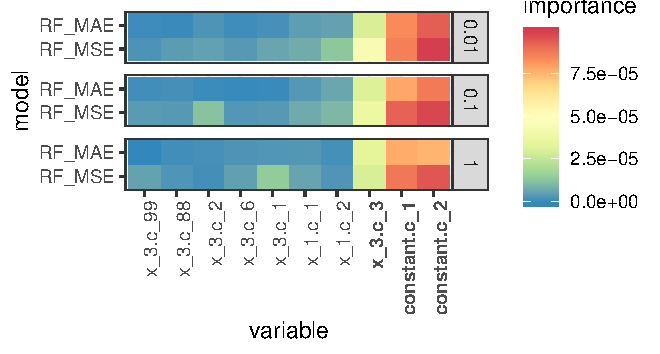
\includegraphics[]{../Results/simulation/graphics/simulation_g1_vimp_bc.pdf}
	\caption{g1 BC VIMP}
\end{figure}

\begin{figure}
	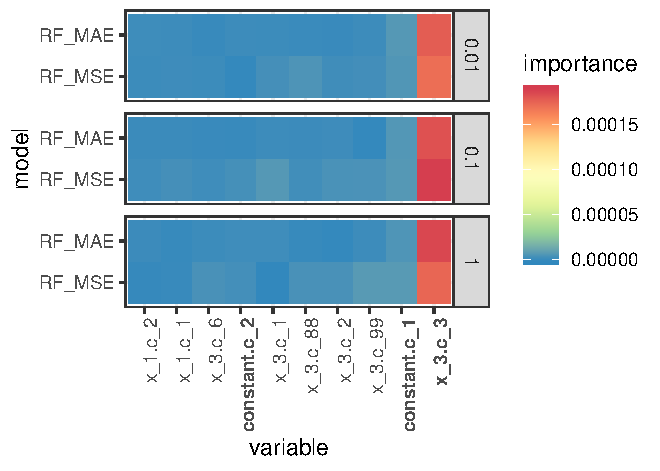
\includegraphics[]{../Results/simulation/graphics/simulation_g2_vimp_bc.pdf}
	\caption{g2 BC VIMP}
\end{figure}

\begin{figure}
	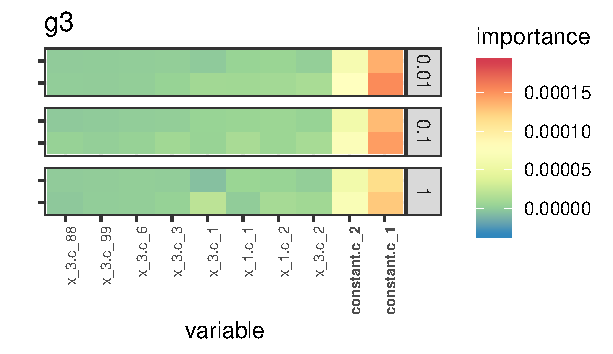
\includegraphics[]{../Results/simulation/graphics/simulation_g3_vimp_bc.pdf}
	\caption{g3 BC VIMP}
\end{figure}

%%IK

\begin{figure}
	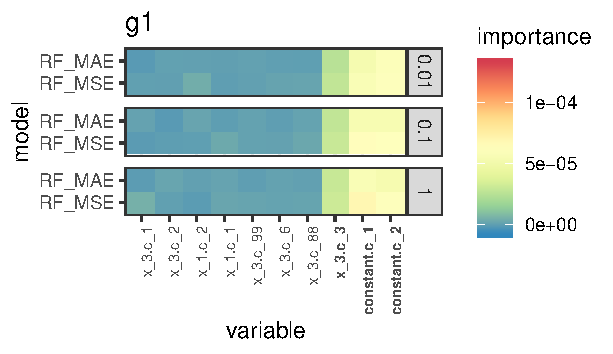
\includegraphics[]{../Results/simulation/graphics/simulation_g1_vimp_ik.pdf}
	\caption{g1 IK VIMP}
\end{figure}

\begin{figure}
	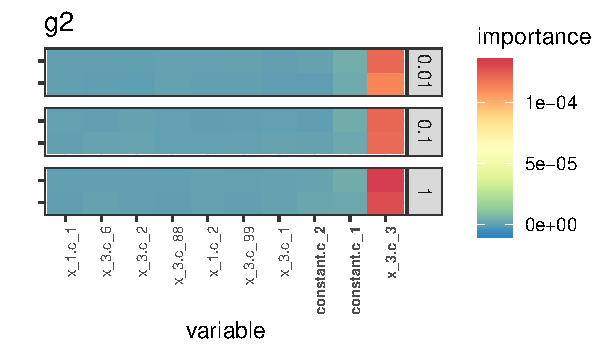
\includegraphics[]{../Results/simulation/graphics/simulation_g2_vimp_ik.pdf}
	\caption{g2 IK VIMP}
\end{figure}

\begin{figure}
	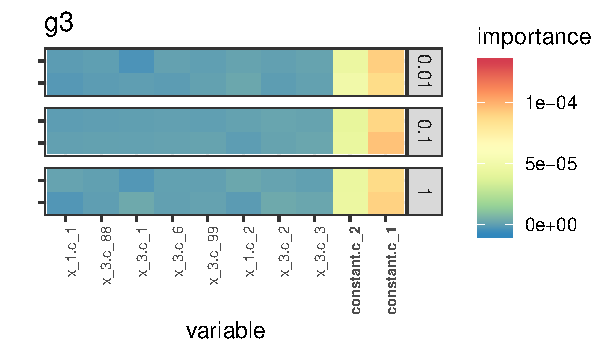
\includegraphics[]{../Results/simulation/graphics/simulation_g3_vimp_ik.pdf}
	\caption{g3 IK VIMP}
\end{figure}

\subsubsection{Empirical Study}
%% Small Results

%% Comprehensive Results

\subsubsection{Empirical Robustness Checks}
%%%%%%%%%%%%%%%%%%%%%%%%%%%%%%%%%%%%%%%%%%
%% Missing Threshold
%%%%%%%%%%%%%%%%%%%%%%%%%%%%%%%%%%%%%%%%%%

%% Loss Stats

%% Factor Importance

%%%%%%%%%%%%%%%%%%%%%%%%%%%%%%%%%%%%%%%%%%
%% Train:Validation 1:1
%%%%%%%%%%%%%%%%%%%%%%%%%%%%%%%%%%%%%%%%%%

%% Loss Stats

%% Factor Importance

%%%%%%%%%%%%%%%%%%%%%%%%%%%%%%%%%%%%%%%%%%
%% Train:Validation 2:1
%%%%%%%%%%%%%%%%%%%%%%%%%%%%%%%%%%%%%%%%%%

%% Loss Stats

%% Factor Importance

%%%%%%%%%%%%%%%%%%%%%%%%%%%%%%%%%%%%%%%%%%
%% Fama French Factors
%%%%%%%%%%%%%%%%%%%%%%%%%%%%%%%%%%%%%%%%%%

%% Loss Stats

%% Factor Importance


%%%%%%%%%%%%%%%%%%%%%%%%%%%%%%%%%%
%%BIBLIOGRAPHY
%%%%%%%%%%%%%%%%%%%%%%%%%%%%%%%%%%

\bibliographystyle{jfe}
\bibliography{Bibliography}

\end{document}